\documentclass{article}
\usepackage{arxiv}

\usepackage[utf8]{inputenc}
\usepackage[english, russian]{babel}
\usepackage[T1]{fontenc}
\usepackage{url}
\usepackage{booktabs}
\usepackage{amsfonts}
\usepackage{nicefrac}
\usepackage{microtype}
\usepackage{lipsum}
\usepackage{graphicx}
\usepackage{natbib}
\usepackage{doi}
\usepackage{amsmath}
\usepackage{hyperref}
\usepackage{caption}
\DeclareMathOperator*{\argmax}{arg\,max}
\DeclareMathOperator*{\argmin}{arg\,min}


\title{Увеличение эффективности подбора гиперпараметров}

\author{ Валентин А. Абрамов \\
	Факультет вычислительной математики и кибернетики\\
	МГУ имени М. В. Ломоносова\\
	%% \AND
	%% Coauthor \\
	%% Affiliation \\
	%% Address \\
	%% \texttt{email} \\
	%% \And
	%% Coauthor \\
	%% Affiliation \\
	%% Address \\
	%% \texttt{email} \\
	%% \And
	%% Coauthor \\
	%% Affiliation \\
	%% Address \\
	%% \texttt{email} \\
}
\date{}

% \renewcommand{\shorttitle}{\textit{arXiv} Template}
% \renewcommand{\abstractname}{Аннотация}
%%% Add PDF metadata to help others organize their library
%%% Once the PDF is generated, you can check the metadata with
%%% $ pdfinfo template.pdf
% \hypersetup{
% pdftitle={A template for the arxiv style},
% pdfsubject={q-bio.NC, q-bio.QM},
% pdfauthor={David S.~Hippocampus, Elias D.~Striatum},
% pdfkeywords={First keyword, Second keyword, More},
% }

\begin{document}
\maketitle

\begin{abstract}
В данной статье предложено улучшение метода дифференциальной эволюции, лежащего в основе DEHB. Алгоритм DEHB жадный -- постоянно переиспользует старые значения. Предложено добавлять шум во время мутации для увеличения покрытия пространства гиперпараметров.
Были представлены экспериментальные результаты, демонстрирующие эффективность этого метода в сравнении с базовым DEHB и традиционными методами выбора гиперпараметров. Результаты показывают, что изменение мутации может обеспечить более высокую точность модели при неизменном использовании вычислительных ресурсов.

\end{abstract}

\keywords{Оптимизация гиперпараметров \and Эволюционный алгоритм}

\section{Введение}

В последние годы машинное обучение стало одной из самых активно развивающихся областей в информационных технологиях. Чтобы достичь высокого качества моделей машинного обучения, необходимо правильно настроить гиперпараметры алгоритмов.

Гиперпараметры являются важными параметрами моделей машинного обучения, которые не могут быть определены в процессе обучения. Традиционные методы выбора гиперпараметров, такие как сеточный поиск \cite{grid_search} или случайный поиск \cite{random_search}, могут быть неэффективными или требовать значительных вычислительных ресурсов, поэтому вместо них используют более сложные алгоритмы, например, эволюционные. Одним из таких алгоритмов является DEHB \cite{awad2021dehb}.


\section{Обзор литературы}

Гиперпараметрическая оптимизация - большая и перспективная область исследований. В статье \cite{bischl2021hyperparameter} приводится подробный обзор существующих методов, все алгоритмы формально описаны, поднимаются вопросы переобучения гиперпараметров на валидационную выборку и параллелизации алгоритмов. Для глубоких нейронных сетей также необходимо подбирать гиперпараметры, такие как число слоёв, learning rate и даже связи между слоями. О задачах гиперпараметрической оптимизации в нейронных сетях подробно написано в статье \cite{Talbi2020OptimizationOD}.

Задача автоматического подбора гиперпараметров активно исследуется (\cite{Liu_2023}, \cite{morales2023survey}). Ранее использовались методы перебора по сетке (\cite{grid_search}) или случайного поиска значений (\cite{random_search}), но эти методы имеют свои недостатки, такие как случайность, проклятие размерности, сложность подбора сетки, медленная скорость работы, невозможность учесть взаимосвязи между гиперпараметрами и зависимость целевой метрики от них. В 2011 году был создан подход SMBO - последовательная оптимизация, основанная на суррогатной функции (\cite{10.1007/978-3-642-25566-3_40}). В качестве суррогатной функции изначально брали гауссовские процессы (\cite{wistuba2018scalable}), но они подходят не для всех задач, так как предназначены только для непрерывных гиперпараметров. Также был придуман алгоритм Succesive Halving (\cite{jamieson2015nonstochastic}), представляющий из себя жадный алгоритм, инкрементально выделяющий больше ресурсов для оценки гиперпараметров с хорошим потенциалом.

На данный момент одним из лучших методов поиска является TPE (\cite{NIPS2011_86e8f7ab}), основанный на байесовском подходе. Также существуют методы, основанные на подходе SMBO, такие как SMAC (\cite{10.1007/978-3-642-25566-3_40}, \cite{lindauer2022smac3}), использующий случайный лес в качестве суррогата, или модели, использующие суррогат на основе гауссовских процессов (\cite{schilling2016scalable}, \cite{wistuba2018scalable}). Также стоит упомянуть об эволюционных алгоритмах (\cite{young2015optimizing}, \cite{alibrahim2021hyperparameter}), так как они позволяют оптимизировать любые функции за счет интеллектуального перебора значений, основанного на таких идеях эволюции, как мутация, селекция и естественный отбор. Лучше всего себя показывают методы, основанные на алгоритме Succesive Halving -- они позволяют найти лучший набор гиперпараметров в условиях ограниченности вычислительных мощностей. На основе SH созданы алгоритмы HyperBand (\cite{li2018hyperband}), автоматически выделяющий ресурсы для нескольких запусков SH, BOHB (\cite{falkner2018bohb}), добавляющий в HyperBand суррогат на основе TPE, и DEHB \cite{awad2021dehb}, добавляющий в HB идею дифференциальной эволюции. 

По текущим бенчмаркам (\cite{vanschoren2014openml}, \cite{zela2020bench}) DEHB является SOTA-алгоритмом подбора гиперпараметров, но у него есть недостатки. Из-за жадного переиспользования оптимальных значений при дифференциальной эволюции, модель застревает в локальном минимуме и целевая метрика выходит на плато. Чтобы этого избежать, необходимо перейти от эксплуатации оптимальных в смысле локального минимума значений и добавить новых кандидатов, отличающихся от эксплуатируемых. 

Предлагается добавлять шумовые векторы в эволюционном шаге. Размер шума может зависеть от количества итераций, меняться от выхода на плато по целевой метрике или быть постоянным как гиперпараметр. Таким образом, благодаря шумовым векторам увеличится покрытие поверхности функции ошибки от гиперпараметров.

Для демонстрации результатов работы предложенного метода будут использованы датасеты с сайта \href{https://www.openml.org/}{open-ml}.


\section{Постановка задачи}
Задача гиперпараметрической оптимизации состоит в том, чтобы имея набор данных $X \in \mathbb{R}^{N\times d}, y \in \mathbb{R}^{N}$, пространство гиперпараметров $\Theta \in \mathbb{R}^k$, модель $f(\theta): \mathbb{R}^{d} \to \mathbb{R},\ \theta \in \Theta$, $f \in \mathbb{H}$ и целевую метрику $c(f, X, y): \mathbb{H} \times \mathbb{R}^{N\times d} \times \mathbb{R}^{N} \to \mathbb{R}$, найти $\theta^*$ такую, что выполнено
$$\theta^* = \argmin_{\theta} c(f(\theta), X, y)$$
Таким образом, зная модель $f$, пространство гиперпараметров $\Theta$, набор данных $X, y$ и целевую метрику $c$, необходимо найти набор гиперпараметров $\theta^*$, при котором целевая метрика $c$ наименьшая при обучении модели $f$ на данных $X, y$.

Предполагается, что набор данных состоит из непрерывных переменных, функция $c$ имеет бюджет вычислений. Им может быть ограничение на максимальное число итераций при обучении нейронной сети, количество деревьев в случайном лесе и градиентном бустинге и т. п.


\section{Базовый метод}
\subsection{Differential Evolution}
Алгоритм дифференциальной эволюции (\cite{de}) -- эволюционный алгоритм для наборов непрерывных переменных. Поколение $g$ состоит из $N$ кандидатов $x_{i, g} = (x_{i,g}^1, x_{i,g}^2, ..., x_{i,g}^D)$. Первое поколение инициализируется кандидатами, сэмплируемыми из равномерного распределения. Для каждого кандидата вычисляется целевая функция $f$. Далее для каждого кандидата $x_{i, g}$ выбираются 3 случайных кандидата  $x_{r_1, g}, x_{r_2, g}, x_{r_3, g}$ и строится вектор-мутант вида $v_{i, g} = x_{r_1, g} + F(x_{r_2, g} - x_{r_3, g})$, $F$ -- число-гиперпараметр метода. Далее на основе объектов $x_{i, g}$ и $v_{i, g}$ строится новый кандидат-отпрыск $u_{i, g}$ по следующей схеме: в j-ой координате нового вектора с вероятностью $p$ выбирается значение $x_{i, g}^j$ и с вероятностью $1 - p$ значение $v_{i, g}^j$, $p$ -- гиперпараметр. Этот шаг называется кроссовером (или кроссинговером). Далее для всех отпрысков вычисляется целевая функция и в качестве следующей популяции выбираются N лучших (в смысле значений целевой функции) кандидатов из всех $x_{i, g}$ и $u_{i, g}$.

\subsection{Succesive Halving}
Succesive Halving (\cite{jamieson2015nonstochastic}) -- алгоритм подбора гиперпараметров, подразумевающий наличие бюджета вычислений. То есть целевую функцию $f$ можно вычислить с фиксированным бюджетом, например, можно ограничить количество итераций вычисления $f$. У алгоритма есть три гиперпараметра: количество начальных кандидатов $N$, минимальный бюджет $\lambda$ и $\eta$ -- параметр скалирования. На первой итерации из равномерного распределения сэмплируются $N$ кандидатов, для них вычисляется функция $f$ с бюджетом $\lambda$. На второй итерации берутся $N/\eta$ лучших кандидатов, для них вычисляется $f$ с бюджетом $\eta\lambda$. На i-ой итерации функция $f$ вычисляется для $N/\eta^{i - 1}$ лучших кандидатов с шага $i - 1$ с бюджетом $\eta^{i - 1}\lambda$. Таким образом, алгоритм дает больше ресурсов перспективным кандидатам и отсекает тех, кто при низком бюджете показывает себя хуже остальных.

\subsection{HyperBand}
HyperBand (\cite{li2018hyperband}) расширяет идеи SH -- производится несколько запусков SH с различными значениями $N$ и $\lambda$. Для каждого нового запуска уменьшается число кандидатов и увеличивается минимальный бюджет. Таким образом, функции $f$, которые долго сходятся, проверяются для случайных инициализаций и с низким бюджетом, и с высоким. Главным минусов SH и HyperBand является то, что они полностью полагаются на случайное сэмплирование.

\subsection{DEHB}
DEHB -- Differential Evolution HyperBand -- развивает идеи HyperBand: сэмплирование из равномерного распределения производится один раз, далее лучшие кандидаты передаются в следующие запуски SH. На каждом шаге SH производится модифицированная дифференциальная эволюция -- текущие кандидаты, полученные из предыдущего запуска SH, скрещиваются с мутантами, полученными с помощью сэмплирования лучших кандидатов с предыдущей итерации текущего запуска SH.

\section{Предлагаемый метод}
У алгоритма DEHB есть недостаток -- он использует случайное сэмплирование всего один раз, и далее кандидаты меняются только за счет дифференциальной эволюции. Алгоритм часто застревает в локальном минимуме и выходит на плато по целевой метрике, что может быть связано с жадным переиспользованием кандидатов, лежащих на маленьком расстоянии друг от друга и имеющим близкие значения метрики. 

Чтобы этого избежать, предлагается добавлять шумовые векторы к мутантам при эволюции. Благодаря шумовым векторам увеличится покрытие поверхности функции ошибки от гиперпараметров. Это приведет к тому, что некоторые наборы гиперпараметров из популяций будут находиться вне локального минимума. При скрещивании с наборами вне локального минимума DEHB сможет найти новые оптимальные решения.

Таким образом, мутант будет иметь вид $v_{i, g} = x_{r_1, g} + F(x_{r_2, g} - x_{r_3, g}) + m(t)\varepsilon$, где $m(t): \mathbb{R} \to \mathbb{R}$ -- множитель при шумовом векторе. $m(t)$ может зависеть от номера итерации и увеличиваться со временем, может зависеть от выхода на плато, и также может быть константой.

Зададим $m(t)$ следующим образом: 
$$
m(t) = \begin{cases}
			b + s, & \text{если модель находится на плато метрики качества}\\
            b, & \text{иначе}
		 \end{cases},$$ 
где $b$ -- базовое значение шума, $s$ -- шаг шума (параметры метода). Выход на плато определяется отсутствием улучшения качества в течение 10 итераций.

\newpage

\section{Вычислительные эксперименты}

\subsection{Исходные данные и условия эксперимента}
Параметры $b, s$ (базовый уровень шума и шаг шума соответственно) подбираются для каждого эксперимента отдельно по запускам с малым количеством прогонов.

Эксперименты проведены на реализации DEHB из библиотеки auto-ml. Для тестирования метода добавлена стратегия мутации noisy1\_bin. В качестве модели для оптимизации гиперпараметров взяты RandomForestClassifier и RandomForestRegressor из библиотеки scikit-learn. 

При тестировании метода с зашумлением, если не оговорено иное, шум равен 0, пока функция потерь не выйдет на плато (последние 10 итераций не будет улучшения значения функции потерь).

Метод тестируется на  данных о недвижимости California Housing из библиотеки scikit-learn и наборах данных с сайта \href{https://www.openml.org/}{open-ml}: \href{https://www.openml.org/search?type=data&sort=runs&status=active&id=31}{credit-g}, \href{https://www.openml.org/search?type=data&status=active&id=1504&sort=runs}{steel plates fault}, \href{https://www.openml.org/search?type=data&status=active&id=312}{scene}.

Наборы данных разбивались на обучающую, тестовую и валидационную выборку в соотношении 7:2:1. В задачах регрессии использовалась функция ошибки MSE, в задачах классификации $1 - \text{accuracy}$ (DEHB минимизирует).

Для каждого датасета выполнено 20 запусков DEHB со стратегией мутации rand1\_bin и 20 запусков с новой стратегией. На графиках линиями изображены средние значения функции ошибки на валидационной выборке для итерации обучения на наборе гиперпараметров. Прозрачные области поверх линий - 95\% доверительный интервал значений ошибки.

\subsection{Эксперименты на наборах данных}

\begin{table}[h]
    \centering
    \begin{tabular}{cc}
        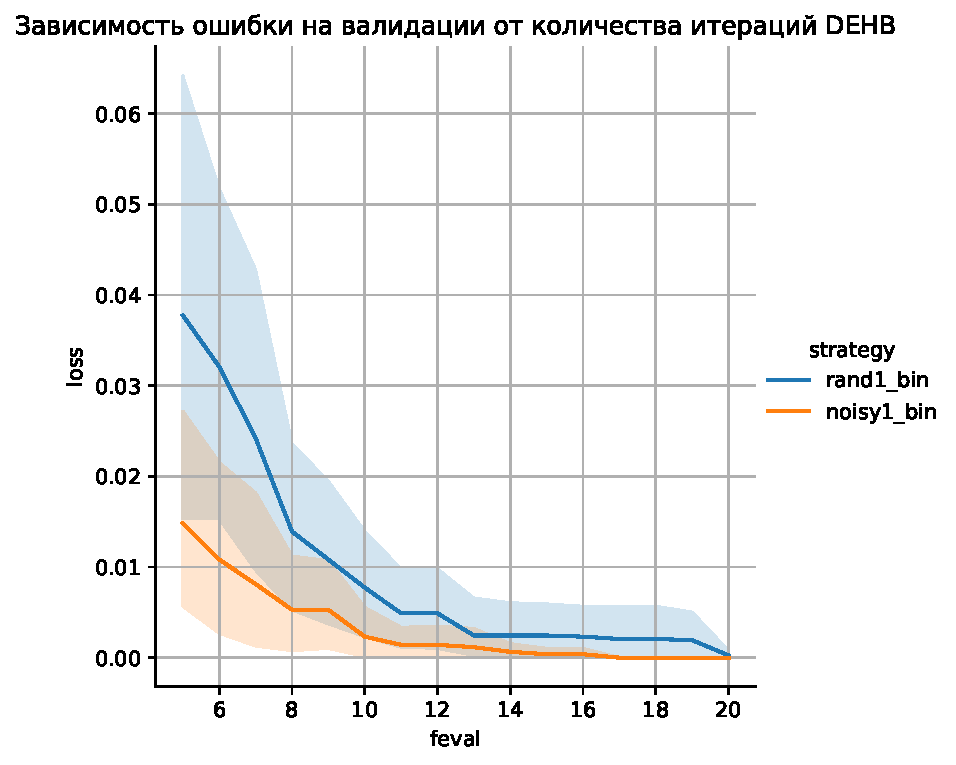
\includegraphics[width=7cm]{steel_plates_cmp.pdf}
        &
        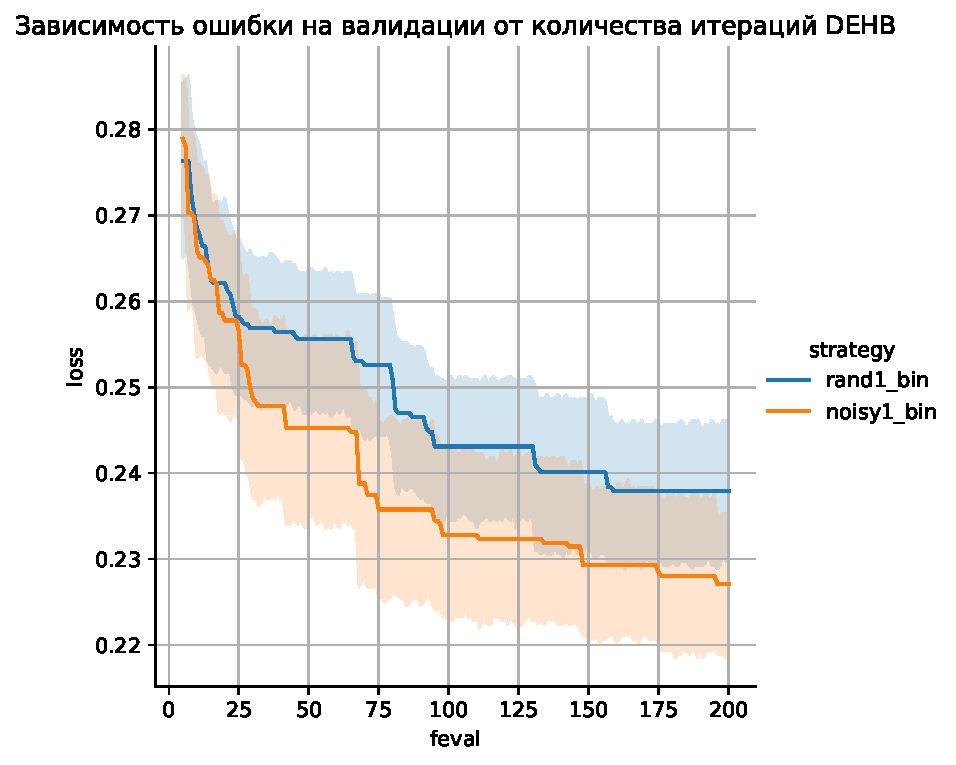
\includegraphics[width=7cm]{liver_cmp.pdf} \\
        Steel plates fault & Liver patients
    \end{tabular}
    \label{table:datasets1}
    \caption{}
\end{table}
\par

В задачах детекции брака стальных пластин и в задаче детекции пациентов с заболеваниями печени предложенный метод стабильно предсказывает лучшие наборы гиперпараметров, чем базовая стратегия мутации. Кроме того, даже несмотря на усреднение ошибок по различным запускам, невооружённым взглядом видно, что базовый метод без зашумления дольше выходит с каждого плато (``ступеньки'' на синем графике длиннее).

\begin{table}[h]
    \centering
    \begin{tabular}{cc}
        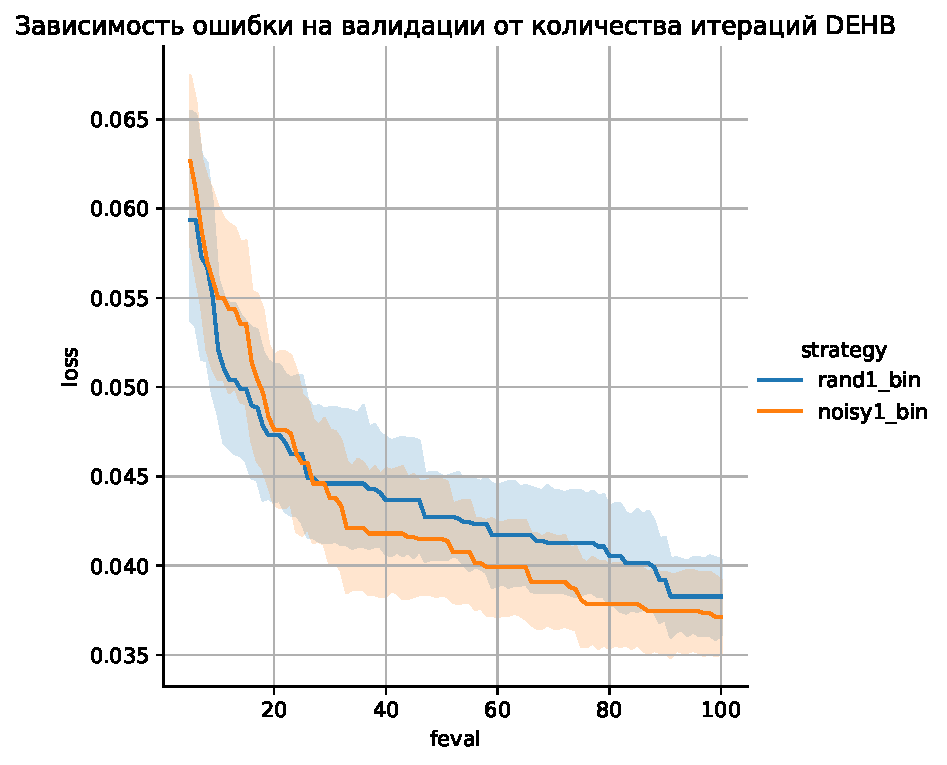
\includegraphics[width=7cm]{scene_cmp.pdf}
        &
        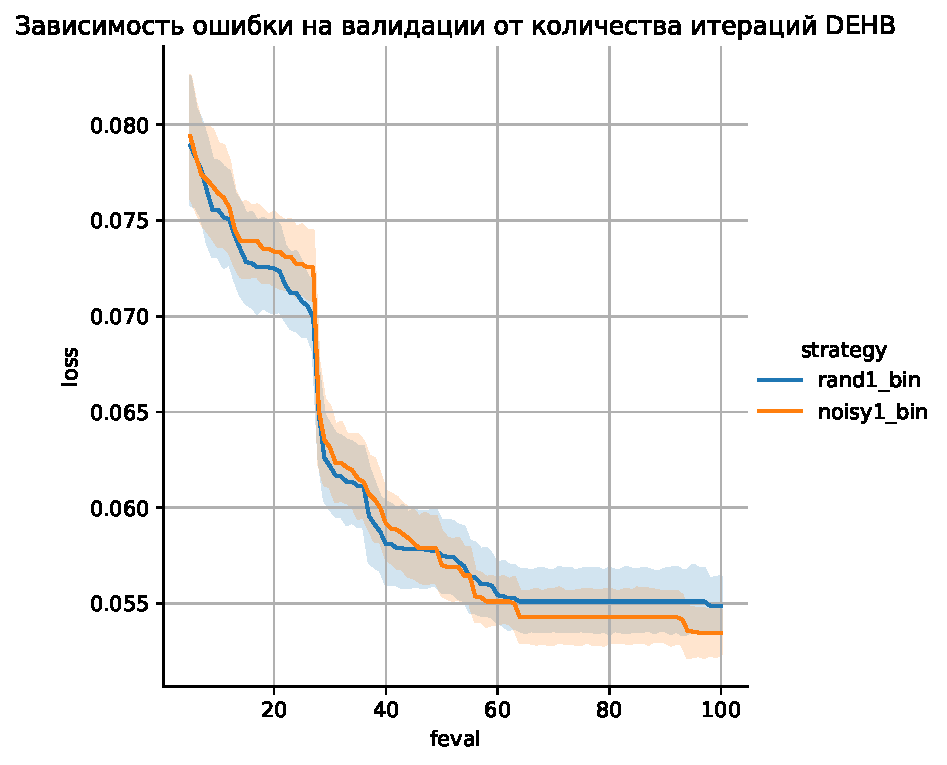
\includegraphics[width=7cm]{spam_cmp.pdf} \\
        Scene detection  & Spam detection
    \end{tabular}
    \label{table:datasets2}
    \caption{}
\end{table}
\par

При тестировании метода на задаче предсказания городcкой среды по эмбеддингам картинки и задаче детекции спама метод показывает менее стабильный прирост качества, однако можно заметить, что предложенный метод действительно выходит с плато быстрее классического.


\newpage

\subsection{Анализ ошибки}
 
Используем датасет с данными о недвижимости для анализа зависимости ошибки метода от его гиперпараметров.
\begin{table}[h]
    \centering
    \begin{tabular}{cc}
        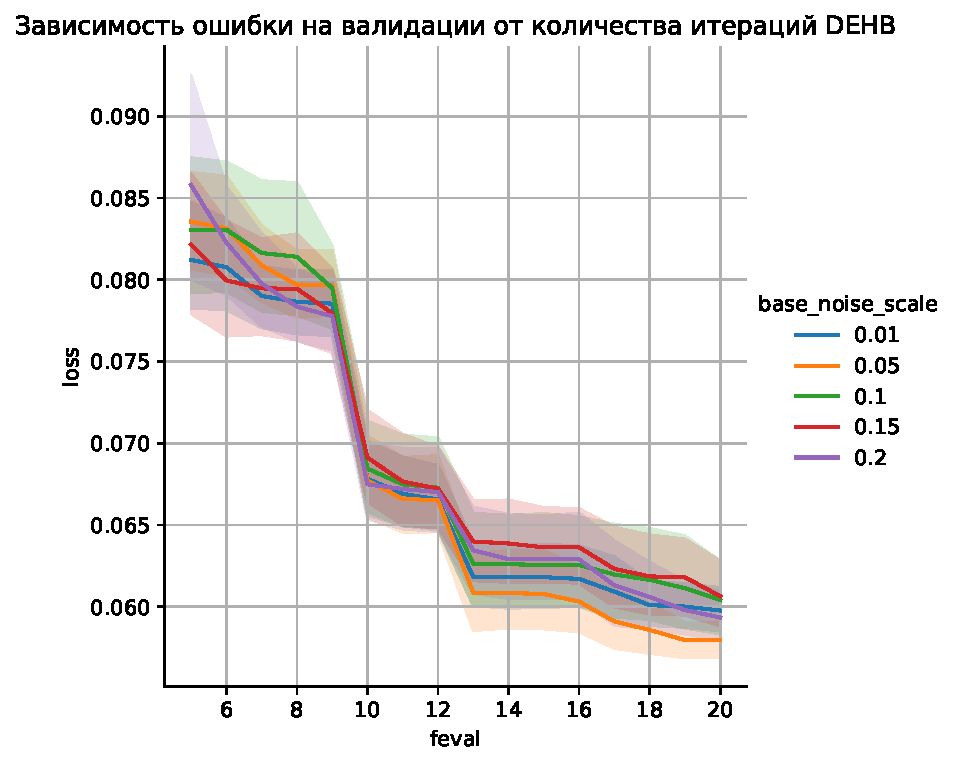
\includegraphics[width=7cm]{cali_housing_ablation.pdf}
        &
        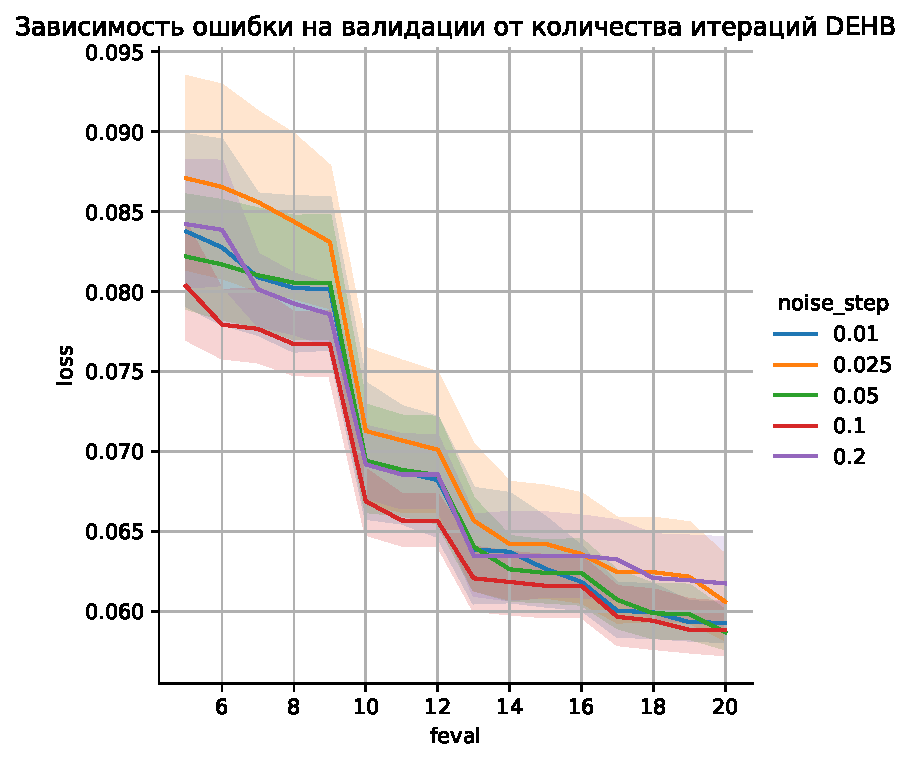
\includegraphics[width=7cm]{cali_housing_step_ablation.pdf} \\
        Зависимость от базового шума & Зависимость от величины шага
    \end{tabular}
    \label{table:datasets2}
    \caption{}
\end{table}
\par
При рассмотрении зависимости от базового шума шаг равнялся 0. Видим, что на малом числе итераций нет значимой зависимости ошибки от параметров метода. Рассмотрим ошибку на задаче детекции пациентов с заболеваниями печени.

\newpage

\begin{table}[h]
    \centering
    \begin{tabular}{cc}
        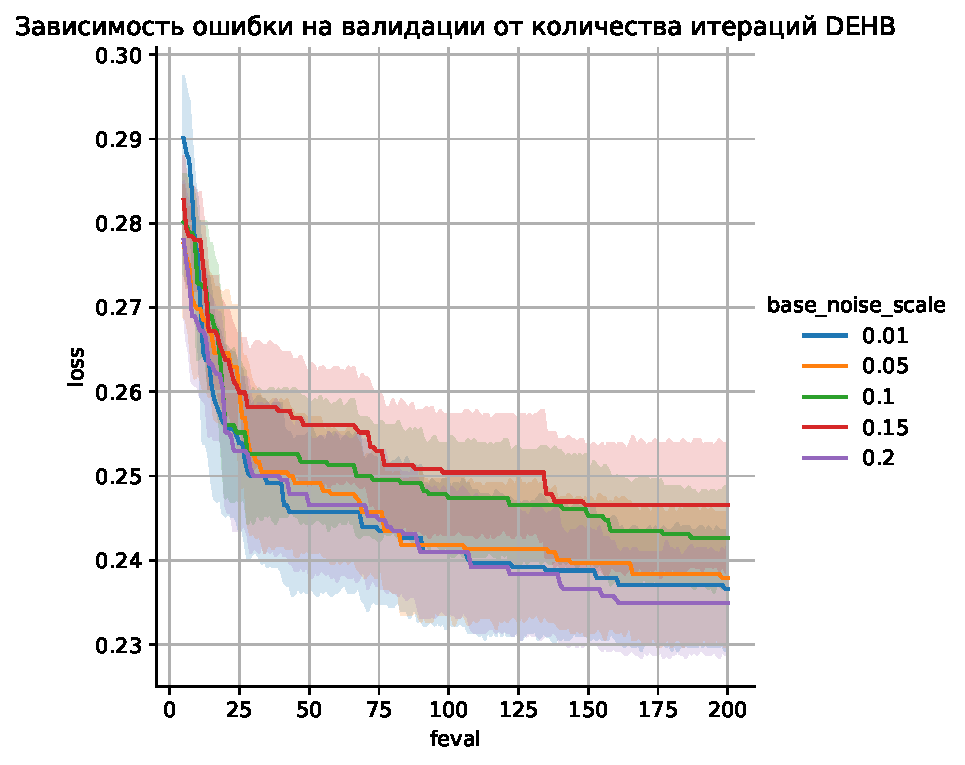
\includegraphics[width=7.3cm]{liver_ablation.pdf}
        &
        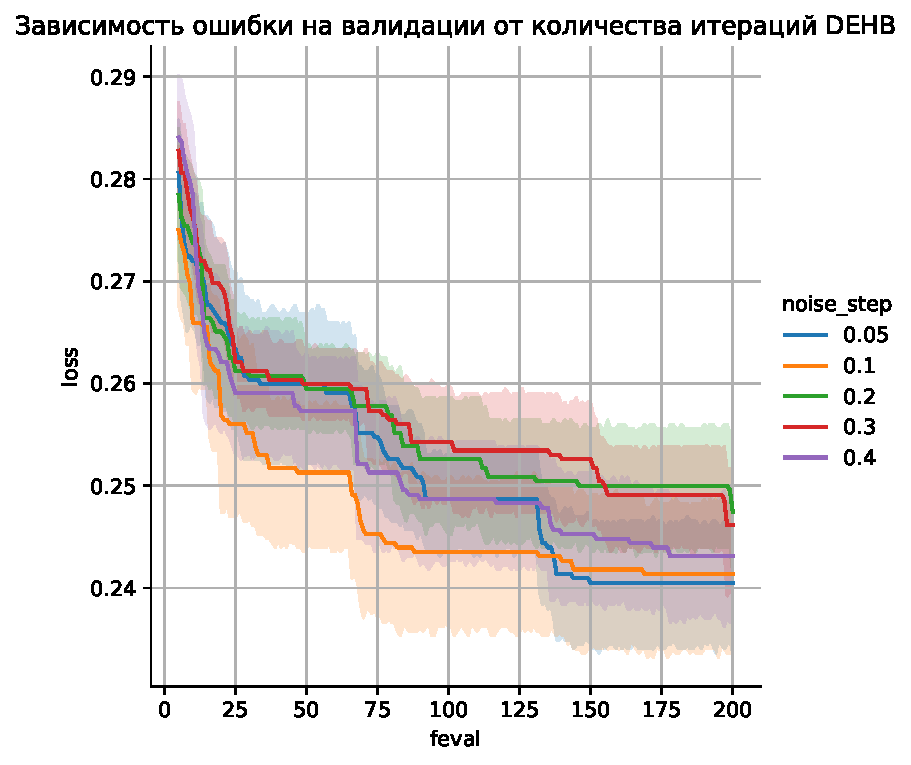
\includegraphics[width=7cm]{liver_step_ablation.pdf} \\
        Зависимость от базового шума & Зависимость от величины шага
    \end{tabular}
    \label{table:datasets2}
    \caption{}
\end{table}
\par
Видим, что явной монотонной зависимости от базового уровня шума нет. При этом на больших уровнях базовго шума модель даже дольше находится на плато, так как новые конфигурации становятся слишком случайными и поиск идет в случайных областях вместо окрестности лучших наборов гиперпараметров.

При рассмотрении зависимости ошибки от величины шага видно, что слишком маленькие и слишком большие величины шага оказывают негативное влияние на ошибку на валидации. Однако видно, что при любых значениях метод позволяет выйти с плато и прийти к новым минимумам функции ошибок.

Также стоит заметить, что параметры метода стоит подбирать в зависимости от размерности пространства гиперпараметров, так как шум одной и той же величины с увеличением размерности будет вносить больший вклад в мутацию.

\section{Выводы}
Таким образом, предложенный метод показывает улучшение на некоторых датасетах. Добавление шума при выходе на плато позволяет получить новых кандидатов и продолжить подбор гиперпараметров с помощью дифференциальной эволюции.

Главной особенностью нового метода является гиперпараметр $m(t)$. Если взять его равным 0, то метод сводится к обычному DEHB. От выбора функции $m(t)$ зависит соотношение exploration/exploitation. При большим уровнях шума мутанты получаются полностью случайными, а при низких -- слишком близкими к кандидатам. Это одновременно является плюсом и минусом метода -- при удачно подобранном $m(t)$ алгоритм сможет быстро уходить с плато, а при неудачном -- покажет себя хуже классического DEHB.

Дальнейшими направлениями исследования являются изучение возможности добавления сэмплирования кандидатов из неисследованных участков пространства гиперпараметров, как это происходит в SMBO. Также можно изменить функции мутации -- например, сдвигать мутанта в направлении увеличения качества целевой метрики. Функцию кроссовера также можно сделать более сложной -- не выбирать одно из двух значений, а брать промежуточное.

\newpage

\bibliographystyle{unsrtnat}
\bibliography{references}

\end{document}